\chapter{Discrete differential geometry and computer graphics}
\label{ch::ddg}

This chapter is divided into three parts. First, we introduce basic notions of \textit{discrete} differential geometry, which correspond to the ideas of ``regular'' differential geometry we seen. The next part relies on the first part, and shows how to ``smooth out a surface'' in a discrete setting by using the Laplacian operator $\Delta$. The third part describes how to take advantage of the complex numbers to set up a minimization problem, that when solved, produces a chart mapping into $\C$ that preserves its manifold's notion of angle as best as possible.

\section{Discrete differental geometry}

In this section, we follow Section 4.8 of \cite{book::DDG}, and translate concepts from ``regular'' differential geometry over to their discrete counterparts. To begin our translation of concepts, we recall that the ``regular'' differential forms of the previous chapter lived on smooth manifolds WWBOC. \textit{Discrete differential forms} will live on \textit{simplicial complexes}, or \textit{meshes}, that are built out of \textit{simplices}.

\begin{defn}
    (Oriented $k$-simplex in $\R^n$).
    
    An \textit{oriented $k$-simplex $k \leq n$, in $\R^n$} is a tuple $(K, \text{Or})$, where $K \subseteq \R^n$ is a subset of the form
    
    \begin{align*}
        \Big\{ \sum_{i = 1}^{k + 1} c_i \qq_i \mid \sum_{i = 1}^{k +1} c_i = 1, c_i \geq 0 \Big\},
    \end{align*}
    
    and where $\text{Or}$ is the standard orientation of $\{\pp_1, ..., \pp_{k + 1} \}$ inherited from $\R^k$.
    
    When treated as a manifold embedded in $\R^n$, an oriented $k$-simplex can be given a smooth structure so that it is a smooth oriented manifold with corners.
\end{defn}

\begin{example}
    ($0$-, $1$-, and $2$- simplices). 
    
    A $0$-simplex is a vertex (a point with positive orientation), a $1$-simplex is an edge (an oriented line segment), a $2$-simplex is an oriented triangle, and a $3$-simplex is an oriented tetrahedron.
\end{example}

\begin{defn}
\label{ch::ddg::defn::mesh}
    (Oriented simplicial $k$-complex in $\R^n$).
    
    An \textit{oriented simplicial $k$-complex in $\R^n$} is a union of oriented $k$-simplices in $\R^n$, where the pairwise intersections have measure zero, such that any two faces that fill the same space are oppositely oriented. 
    
    We often refer to an oriented simplicial $k$-complex in $\R^n$ as a \textit{$k$-mesh}, or simply as a \textit{mesh}.
\end{defn}

Now that the setting for discrete differential forms has been established, we move to define discrete differential forms themselves. \cite{DDGArticle} notes that ``finding a discrete counterpart to the notion of differential forms is a delicate matter. If one was to represent differential forms using their coordinate values and approximate the exterior derivative using finite differences, basic theorems such as Stokes’ theorem would not hold numerically''. Recognizing this issue, we now present a definition of discrete differential $k$-form that \textit{does} work.

\begin{defn}
    (Discrete differential $k$-form).
    
    Let $K$ be a $k$-mesh, considered as a smooth $k$-manifold with corners embedded in $\R^n$, and let $\omega$ be a differential $k$-form on $K$. We define the \textit{discrete differential $k$-form $\homega$ on $K$ corresponding to $\omega$} to be the function which integrates $\omega$ over an arbitrary collection of $k$-simplices in $K$. That is, if $\{K_i\}$ is a finite collection of $k$-simplices in $K$, then the \textit{evaluation $\homega_{\{K_i\}}$ of $\homega$ on $\{K_i\}$} is defined to be
    
    \begin{align*}
        \homega_{\{K_i\}} := \int_{\{K_i\}} \omega = \sum_i \int_{K_i} \omega.
    \end{align*}
    
    Here, the hat $\spc\widehat{\spc}\spc$ is meant to denote ``discrete'', \textit{not} ``normalized''.
\end{defn}

\begin{defn}
    (Convention for discrete $0$-forms).
    
    By the previous definition, a discrete $0$-form is a $0$-form (i.e. a function) that's been integrated over every $0$-simplex in a $1$-simplex. The integral of a function ``over'' a point is zero, but we will use the convention of treating the value of a discrete $0$-form $\hf|_{\pp_i}$ at a point to be the value of the corresponding function at that point, $\hf|_{\pp_i} := f|_{\pp_i}$.
\end{defn}

Now that we have defined discrete differential forms, we expect a corresponding definition of discrete exterior derivative.

\begin{defn}
    (Discrete exterior derivative).
    
    Let $K$ be a $k$-mesh, and consider a discrete differential $\ell$-form $\homega$, $\ell < k$, on $K$.
    The \textit{discrete exterior derivative} $\hd$ acts on $\homega$ to produce a discrete differential $(\ell + 1)$-form $\hd \homega$ on $K$. The value of $\hd \homega$ at an $(\ell + 1)$-simplex $L$ of $K$ is given by
    
    \begin{align*}
        (\hd\homega)_L := \int_L d \omega.
    \end{align*}
\end{defn}

The following theorem reveals why we chose to define the discrete exterior derivative as we did.

\begin{theorem}
\label{ch::ddg::thm::discrete_stokes}
    (Stokes' theorem for discrete differential forms).
    
    If the $(\ell + 1)$-simplex $L$ of the previous definition is the finite union of $\{L_i\}$, where the pairwise intersections of the $\{L_i\}$ have measure zero, then we have
    
    \begin{align*}
        (\hd\homega)_L = \int_L d \omega = \int_{\pd L} \omega = \sum_i \int_{(\pd L)_i} \omega = \sum_i \homega_{(\pd L)_i}.
    \end{align*}
    
   (We have assumed existence of a finite collection $\{(\pd L)_i\}$, where the pairwise intersections of $\{(\pd L)_i\}$ have measure zero, whose union is $\pd L$).
    
    Thus, we have recovered a discrete version of Stokes' theorem:
    
    \begin{align*}
        \boxed
        {
            (\hd\homega)_L = \sum_i \homega_{(\pd L)_i}
        }
    \end{align*}
\end{theorem}

\begin{example}
    (Computing the discrete exterior derivative).
    
    \begin{figure}[H]
        \centering
        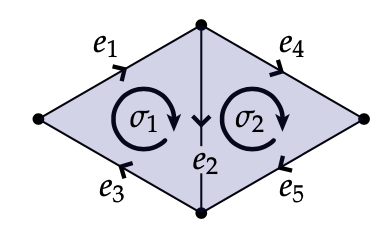
\includegraphics{images/Discrete_exterior_deriv_orientation.png}
    \end{figure}
    
    In the above figure, take $\pp_1$ to be the leftmost vertex and $\pp_2$ to be the topmost vertex. We have
    
    \begin{align*}
        (\hd\homega)_{\pp_1} &= \homega_1 + \homega_2 + \homega_3 \\
        (\hd\homega)_{\pp_2} &= \homega_4 + \homega_5 - \homega_1.
    \end{align*}
\end{example}

Before introducing the notion of \textit{mesh duality}, we need to know what a ``$k$-cell in $\R^n$'' is.

\begin{defn}
    ($k$-cell in $\R^n$).
    
    A \textit{$k$-cell in $\R^n$} is a subset of $\R^n$ that is a Cartesian product of $k$ closed intervals.
\end{defn}

\begin{defn}
    \scriptsize \cite{DDGArticle} \normalsize (Mesh duality).
    
    Consider a mesh $L$ (recall Definition \ref{ch::ddg::defn::mesh}). We will consider $L$ to be the ``original'', or \textit{primal mesh}. The \textit{dual mesh} to the primal mesh that is $L$ is obtained by replacing each $k$-simplex in $L$ with an $(n - k)$-cell. As stated in \cite{DDGArticle}, the dual mesh ``inherits several properties and operations'' from the primal mesh. ``Most important is the notion of incidence. For instance, if two primal edges are on the same primal face, then the corresponding dual faces are incident, that is, they share a common dual edge (which is the dual of the primal common face)''.
    
    Since a dual mesh is constructed out of $(n - k)$-cells rather than $(n - k)$-simplices, dual meshes are not necessarily simplicial complexes, but are instead examples of what are called \textit{cell complexes}. 
\end{defn}

\begin{defn}
    \scriptsize \cite{DDGNotes} \normalsize (Dual mesh conventions).

    The previous definition gives topological rules for constructing the dual complex, but it does not specify where the dual cells are located in space. As is done in \cite{DDGNotes}, ``we’ll choose the dual vertices to be located at the circumcenter of their primal face counterparts (circumcenter is the center of the circle that passes through all three triangle vertices)''. Doing this ensures that a dual edge is perpendicular to its corresponding primal edge.
\end{defn}

As it deals with relating $k$-dimensional space to $(n - k)$-dimensional space, the above definition is reminiscent of Hodge-duality. The Hodge-dual is indeed what will establish a correspondence between so-called \textit{primal discrete differential forms} and \textit{dual discrete differential forms}. 

\begin{defn}
\label{ch::ddg::defn::discrete_hodge_dual}
    \scriptsize \cite{DDGNotes} \normalsize (Discrete Hodge-duals)
    
    Let $K$ be a $2$-mesh embedded in $\C$. Denote the $2$-simplices (faces) of $K$ by $F_i$, the $1$-simplices (edges) of $K$ by $e_i$, and the $0$-simplices (vertices) of $K$ by $\pp_i$. We define the \textit{discrete Hodge-dual} $\hst$ on discrete primal differential forms in a piecewise manner:
    
    \begin{align*}
        (\hst \homega)_{F_i} &= \frac{1}{|F_i|} \homega, \quad \quad \text{$\homega$ is a discrete primal differential $2$-form}\\
        (\hst \homega)_{e_i} &= \frac{|e_i^*|}{|e_i|} \homega, \quad \quad \text{$\homega$ is a discrete primal differential $1$-form} \\
        (\hst \hf)_{\pp_i} &= |\pp_i^*| \homega, \quad \quad \text{$\hf$ is a discrete primal differential $0$-form (i.e. a function)}
    \end{align*}

    In the above, $|\cdot|$ takes the volume of its argument (so, in the above, it only ever returns $2$-dimensional area or the length of an edge), $e_i^*$ is the dual edge to $e_i$ (so $e_i^*$ is really a $1$-cell in the dual mesh), and $\pp_i^*$ is the dual vertex to $\pp_i$ (so $\pp_i^*$ is really a $2$-cell in the dual mesh).
    
    The middlemost definition of $\hst$ (which acts on a discrete primal differential $1$-form) is often referred to as the \textit{diagonal Hodge-dual}.
\end{defn}

\newpage

\section{Smoothing with the Laplacian}

In this section, our goal is to discretize the PDE

\begin{align*}
    \frac{\pd \FF}{\pd t} = \Delta \FF,
\end{align*}

where $M$ is a smooth $2$-manifold embedded in $\R^3$, $\FF:M \rightarrow \R^3$ is sufficently smooth, and where the \textit{Laplacian} operator $\Delta$ on vector-valued functions is defined as

\begin{align*}
    \Delta \FF = \Delta \begin{pmatrix} F_1 \\ F_2 \\ F_3 \end{pmatrix} := \begin{pmatrix} \Delta F_1 \\ \Delta F_2 \\ \Delta F_3 \end{pmatrix}.
\end{align*}

Here, the $\Delta$ on the right hand side of this definition is the Laplacian operator on scalar-valued functions, $\Delta = \div \circ \grad$.

It can be shown that $\Delta \FF = 2H\hat{\nn}$, where $H$ is the mean curvature\footnote{There are various ways to measure the curvature of a surface at a point. The mean curvature is one of these ways.} and $\hat{\nn}$ is the unit normal (see \cite[p. 114]{book::DDG}). Thus $\FF$ satisfies the above PDE iff, one can stay on the surface by going in the direction of the normal at a point, with strength proportional to the mean curvature at that point. More briefly, solving the above PDE is a formal way to ``smooth out'' the surface $M$ parameterized by $\FF$.

In order to solve the PDE $\frac{\pd \FF}{\pd t} = \Delta \FF$, we will set $\GG := \Delta \FF$ and consider the more abstract problem of

\begin{align*}
    \Delta \FF
    =
    \begin{pmatrix} \Delta F_1 \\ \Delta F_2 \\ \Delta F_3 \end{pmatrix}
    =
    \begin{pmatrix} G_1 \\ G_2 \\ G_3 \end{pmatrix}
    =
    \GG.
\end{align*}

This problem further reduces to the problem $\Delta F_i = G_i$, that is,

\begin{align*}
    \Delta f = g,
\end{align*}

where $f, g:M \rightarrow \R$ are sufficiently smooth real valued functions on $M$. So, our goal has turned into discretizing the Laplacian $\Delta$ on scalar-valued functions.

\subsection*{Discretizing the Laplacian}

We present two approaches for turning the ``regular'' Laplacian operator $\Delta$ on scalar-valued fucntions into the discrete Laplacian operator $\hDelta$ on scalar valued functions. The relatively standard first approach is to use the \textit{finite element method}. The novel second approach utilizes discrete differential geometry.


\subsubsection*{Discretizing the Laplacian with the finite element method}

Consider the PDE

\begin{align*}
    \Delta f = g.
\end{align*}

The basic of the idea of the \textit{finite element method} is to consider ``approximate solutions'' to the PDE in question that are defined piecewise on finitely many regions, called \textit{elements}. The vector space of functions that are defined piecewise on elements is called the \textit{discrete approximation space}. The best \textit{approximate solution} is the function in the discrete approximation space that has the smallest normed \textit{residual}. The norm we use to measure ``normed residuals'' is induced by an inner product on the discrete approximation space.

For our particular problem, our functions are defined on a $2$-mesh $K$ embedded in $\R^3$ (recall Definition \ref{ch::ddg::defn::mesh}). We take the elements to be $2$-simplices on the mesh. Thus, our discrete approximation space is the vector space of sufficiently smooth functions that are defined piecewise on $2$-simplices. 

For the purpose of establishing a norm, we will use the \textit{$L^2$ inner product} $\langle \cdot, \cdot \rangle$ on functions in our discrete approximation space, defined by

\begin{align*}
    \langle f, g \rangle = \int_K fg.
\end{align*}

The residual of a function $h$ in our discrete approximation space is $\Delta h - g$. (The residual is the zero function when $h$ is a solution to the PDE). The normed residual of $h$ is $||\Delta h - g||$, where the norm $||\cdot||$ is induced by the $L^2$ inner product.

In the finite element method, one also makes use of a basis for the discrete approximation space. We will use the basis $\Phi = \{\phi_{\pp_i}\}_{i = 1}^n$ of \textit{hat functions}, where the hat function $\phi_{\pp_i}:K \rightarrow \R$ is defined to be $1$ at the vertex $\pp_i$ and $0$ everywhere else. 

%We will suppose that the minimal possible residual for this particular PDE is $0$. If this is the case, then the best approximation $\hbest$ in the discrete approximation space satisfies $||\Delta \hbest - g||^2 = \langle \Delta \hbest - g, \Delta \hbest - g \rangle = 0$. Since $\Delta \hbest - g$ is in the discrete approximation space, it can be expressed as a basis sum of the hat functions $\phi_{\pp_i}$. We expand the second $\Delta \hbest - g$ in the inner product $ \langle \Delta \hbest - g, \Delta \hbest - g \rangle$ and use linearity, and the fact that sums of nonnegative terms are zero only if all the terms are zero, to obtain that we must have $\langle \Delta \hbest - g, \phi_{\pp_i} \rangle = 0$ for all $i$. That is, the $L^2$ inner product of the residual of the best approximate solution with each hat function is zero.

To discretize the Laplacian operator $\Delta$, we determine the Laplacian of a function $h$ in the discrete approximation space by using the basis of hat functions. We need the following lemma before doing so.

\begin{lemma}
\label{ch::ddg::lemma:green_first_identity}
    (Green's first identity).
    
    Let $M$ be a smooth $2$-manifold embedded in $\R^3$. If $f, g:M \rightarrow \R$ are sufficiently smooth, then
    
    \begin{align*}
        \langle \Delta f, g \rangle = -\langle \nabla f, \nabla g \rangle + \langle \nabla f \cdot \hat{\nn}, g \rangle_\pd,
    \end{align*}
    
    where $\langle \cdot, \cdot \rangle_\pd$ is the $L^2$ inner product on the boundary $\pd K$, and where we've made use of the $L^2$ inner product on vector fields that is defined by
    
    \begin{align*}
        \langle \VV_1, \VV_2 \rangle := \int \VV_1 \cdot \VV_2,
    \end{align*}
    
    Here, $\VV_1 \cdot \VV_2$ denotes the function $\pp \mapsto \VV_1|_\pp \cdot \VV_2|_\pp$.
\end{lemma}

\begin{proof}
    In general, $d(f\omega) = df \wedge d\omega + fd\omega$. So $d(g * df) = dg \wedge *df + gd*df$. Integrate over $M$ and apply Stokes' theorem to the left hand side to obtain
    
    \begin{align*}
        \int_{\pd M} g * df = \int_M dg \wedge *df + \int_M g d*df.
    \end{align*}
    
    Another general fact is that $**\omega = -1^{k(n-k)} \omega$ (see \cite{HodgeStar} for a proof of this), so $**(d*df) = d*df$ (use $k = 3$, $n = 3$). That is, $(d*d)f = *(*d*d)f = * \Delta f$. So the above becomes
    
    \begin{align*}
        \int_{\pd M} g * df =  \int_M dg \wedge *df + \int_M g *\Delta f.
    \end{align*}
    
    This is the same as
    
    \begin{align*}
        \int_{\pd M} g*df = \langle dg, df \rangle + \langle g, \Delta f \rangle.
    \end{align*}
    
    Rearranging, we have
    
    \begin{align*}
        \langle \Delta f, g \rangle = - \langle df, dg \rangle + \int_{\pd M} g*df.
    \end{align*}
    
    To complete the proof, observe that $\langle df, dg \rangle = \langle \nabla f, \nabla g \rangle$, and that after identifying $dx^{\sigma(i)} \wedge dx^{\sigma(j)}$ in $*df$ with $\sgn(\sigma) \see_{\sigma(\{1, 2, 3\} - \{i, j\})}$, $*df$ becomes $\nabla f \cdot \hat{\nn}$.
\end{proof}

We are now ready to take the first step in computing a discretization of the Laplacian with the finite element method.

\begin{deriv}
\label{ch::ddg::deriv::discrete_laplacian_inner_prod_grad}
    (Discrete Laplacian in terms of $L^2$ inner products of gradients).
    
    Let $K$ be a $2$-mesh embedded in $\R^3$, and let $K_j$ be the $2$-simplices (the triangles) on $K$. Using the bilinearity of the inner product $\langle \cdot, \cdot \rangle$, we see the \textit{discretization (via the finite element method) $\hDelta$ of the Laplacian $\Delta$} satisfies

    \begin{align*}
        \langle \hDelta h, \phi_{\pp_i} \rangle 
        = \sum_j \langle \hDelta h, \phi_{\pp_i} \rangle_{K_j}.
    \end{align*}
    
    Applying Green's first identity to the argument of the sum yields
    
    \begin{align*}
        \langle \hDelta h, \phi_{\pp_i} \rangle = -\sum_j \langle \hnabla h, \hnabla \phi_{\pp_i} \rangle_{K_j} + \sum_j \langle \hat{\nn} \cdot \hnabla h, \phi_{\pp_i} \rangle_{\pd K_j}.
    \end{align*}
    
    If the mesh has no boundary, then the inner product on the boundary $\langle \cdot, \cdot \rangle_{\pd K_j}$ vanishes, and we're left with
    
    \begin{align*}
        \langle \hDelta h, \phi_{\pp_i} \rangle = -\sum_j \langle \hnabla h, \hnabla \phi_{\pp_i} \rangle_{K_j}
        = - \langle \hnabla h, \hnabla \phi_{\pp_i} \rangle.
    \end{align*}
    
    Expanding $h$ in the basis $\Phi = \{\phi_{\pp_i}\}_{i = 1}^n$ as $h = \sum_j ([h]_\Phi)_j \phi_{\pp_j}$, using the linearity of $\hnabla$, and using the bilinearity of $\langle \cdot, \cdot \rangle$, we have
    
    \begin{align*}
         \langle \hDelta h, \phi_{\pp_i} \rangle =
         \langle \hnabla \Big( \sum_j ([h]_\Phi)_j \phi_{\pp_j} \Big), \hnabla \phi_{\pp_i} \rangle
         = \sum_j ([h]_\Phi)_j \langle \hnabla \phi_{\pp_j}, \hnabla \phi_{\pp_i} \rangle.
    \end{align*}
\end{deriv}

So it remains to compute $\langle \hnabla \phi_{\pp_j}, \hnabla \phi_{\pp_i} \rangle$. This will be accomplished by the next several lemmas.

\begin{lemma}
\label{ch::ddg:lemma::cotan_w_h_lemma}

    (Cotan formula lemma 1).
    
    The ``aspect ratio'' $\frac{w}{h}$ of a triangle is the sum of the cotangents of the interior angles at its base. That is,
    
    \begin{align*}
        \frac{w}{h} = \cot(\alpha) + \cot(\beta).
    \end{align*}
    
    \begin{figure}[H]
        \centering
        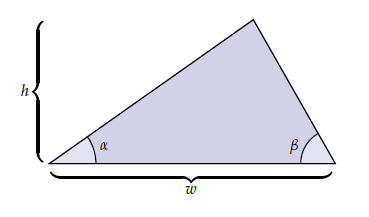
\includegraphics{images/fem_cotan_lemma1.PNG}
        \caption{\cite[p. 105]{book::DDG}}
    \end{figure}
\end{lemma}

\begin{proof}
    Drop an altitude from the top vertex of the triangle so that it intersects the base. Let $x$ denote the length from this intersection point to the right vertex of the triangle. Then $\cot(\alpha) = \frac{w - x}{h}$ and $\cot(\beta) = \frac{x}{h}$, so $\cot(\alpha) + \cot(\beta) = \frac{w}{h}$.
\end{proof}


\begin{lemma}
\label{ch::ddg:lemma::cotan_edge_perp}
    (Cotan formula lemma 2).
    
    If $\ee$ is the edge vector along the base of a triangle, and $\ee_\perp$ is the result of rotating $\ee$ counterclockwise by $\frac{\pi}{2}$, then the gradient of the hat function $\phi$ associated with the vertex opposite the side corresponding to $\ee$ is
    
    \begin{align*}
        \hnabla \phi  = \frac{\ee_\perp}{2A},
    \end{align*}
    
    where $A$ is the area of the triangle.
    
    \begin{figure}[H]
        \centering
        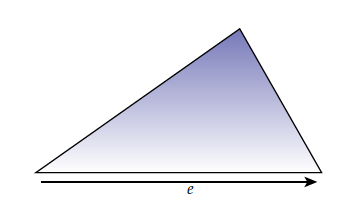
\includegraphics{images/fem_cotan_lemma2.PNG}
        \caption{\cite[p. 106]{book::DDG}}
    \end{figure}
\end{lemma}

\begin{proof}
%http://www.it.uu.se/edu/course/homepage/finmet2/vt14/material/Lab1.pdf
    Denote the left, top, and right vertices of the triangle by $\xx_i$, $i = 1, 2, 3$, respectively. Let $\phi = \phi_2$ denote the hat function associated with $\xx_2$, the top vertex. We have $\phi(\xx_1) = \phi(\xx_3) = 0$ and $\phi(\xx_2) = 1$.
    
    Since $\phi$ is linear, it is of the form $\phi(\xx) = \phi(\pp) + (\hnabla_\xx \phi)|_\pp \cdot (\xx - \pp)$, for any $\pp \in \R^3$. (Here, $\cdot$ is the dot product). It follows that the gradient of $\phi$ is the constant function $\hnabla_\xx \phi \equiv (\hnabla_\xx \phi)|_\pp$. Using $\pp = \xx_2$, we have
    
    \begin{align*}
        \phi(\xx) = 1 + (\hnabla_\xx \phi)|_{\xx_2} \cdot (\xx - \xx_2).
    \end{align*}
    
    Now use $\xx = \xx_1$ and $\xx = \xx_3$ to obtain
    
    \begin{align*}
        0 &= 1 + (\hnabla_\xx \phi)|_{\xx_2} \cdot (\xx_1 - \xx_2) \\
        0 &= 1 + (\hnabla_\xx \phi)|_{\xx_2} \cdot (\xx_3 - \xx_2).
    \end{align*}
    
    These equations are equivalent to
    
    \begin{align*}
        1 &= (\hnabla_\xx \phi)|_{\xx_2} \cdot (\xx_2 - \xx_1) \\
        1 &= (\hnabla_\xx \phi)|_{\xx_2} \cdot (\xx_2 - \xx_3).
    \end{align*}
    
    Subtract the second equation from the first and use the linearity of $\hnabla_\xx$ to obtain
    
    \begin{align*}
        (\hnabla_\xx \phi)|_{\xx_2} \cdot (\xx_3 - \xx_1) &= 0.
    \end{align*}
    
    Thus, $(\hnabla_\xx \phi)|_{\xx_2}$ is perpendicular to $\ee = \xx_3 - \xx_1$, which is the edge vector of the base of the depicted triangle. Since $(\hnabla_\xx \phi)|_{\xx_2}$ is the direction of  greatest \textit{increase}, not decrease, in $\phi$, then $(\hnabla_\xx \phi)|_{\xx_2}$ must point \textit{into} the triangle rather than out. ($\phi$ increases as we go ``into'' the triangle, since ${\phi(\xx_1) = \phi(\xx_3) = 0 < \phi(\xx_2) = 1}$). This implies that the direction of $(\hnabla_\xx \phi)|_{\xx_2}$ is the same as the direction of the $\ee_\perp$ described in the theorem. 
    
    To complete the proof, we will find the magnitude of $(\hnabla_\xx \phi)|_{\xx_2}$ and then show $\hnabla_\xx \phi \equiv (\hnabla_\xx \phi)|_{\xx_2} = \frac{\ee_\perp}{2A}$.
    
    Consider the previous equation
    
    \begin{align*}
        1 &= (\hnabla_\xx \phi)|_{\xx_2} \cdot (\xx_2 - \xx_1).
    \end{align*}
    
    The dot product on the right hand side can be re-expressed as
    
    \begin{align*}
        1 &= ||(\hnabla_\xx \phi)|_{\xx_2}|| \spc ||\xx_2 - \xx_1|| \cos \Big( \frac{\pi}{2} - \alpha \Big),
    \end{align*}
    
    where $\alpha$ is the angle between $(\hnabla_\xx \phi)|_{\xx_2}$ and $\xx_2 - \xx_1$. Equivalently, $\alpha$ is the angle between $\ee$ and the left side of the triangle. Using this reinterpretation of $\alpha$, we solve for $||(\hnabla_\xx \phi)|_{\xx_2}||$ and get
    
    \begin{align*}
        ||(\hnabla_\xx \phi)|_{\xx_2}|| 
        = \frac{1}{||\xx_2 - \xx_1|| \cos\Big( \frac{\pi}{2} - \alpha \Big)}
        = \frac{1}{||\xx_2 - \xx_1|| \sin(\alpha)} = \frac{1}{h},
    \end{align*}
    
    where $h$ is the height of the triangle. 
    
    Putting everything together, and using that $||\ee_\perp|| = ||\ee||$, we have
    
    \begin{align*}
        \hnabla_\xx \phi \equiv (\hnabla_\xx \phi)|_{\xx_2} 
        = ||(\hnabla_\xx \phi)|_{\xx_2}|| \hat{\ee}_\perp 
        = ||(\hnabla_\xx \phi)|_{\xx_2}|| \frac{\ee_\perp}{||\ee_\perp||}
        = \frac{1}{h ||\ee||} \ee_\perp
        = \frac{1}{2(\frac{1}{2} h ||\ee||)} \ee_\perp
        = \frac{\ee_\perp}{2A}.
    \end{align*}
    
    
    %Denote the hat functions associated with these vertices by $\phi_{\pp_i}$, $i = 1, 2, 3$, and suppose $\phi_{\pp_i}(x, y) = a_i + b_ix + c_iy$ for some constants $a_i, b_i, c_i$. By definition of the notion of ``hat function'', we have $\phi_{\pp_i}(\xx_j) = \delta^i_j$, so $a_i, b_i, c_i$ are determined as
    
    %\begin{align*}
    %    \begin{pmatrix}
    %        1 & x_1 & y_1 \\
    %        1 & x_2 & y_2 \\
    %        1 & x_3 & y_3
    %    \end{pmatrix}
    %    \begin{pmatrix} a_i \\ b_i \\ c_i \end{pmatrix}
    %    =
    %    \see_i,
    %\end{align*}
    
    %where $\see_i \in \R^3$ is the $i$th standard basis vector for $\R^3$. 
    
    %We are interested in the hat function $\phi = \phi_2$ corresponding to the top vertex. Solving the above system, we find

    %\begin{align*}
    %    \phi(x, y) = \frac{1}{2A}\Big( (x_3 y_1 - x_1 y_3 ) + (y_3 - y_1)x + (x_1 - x_3)y \Big),
    %\end{align*}
    
    %where $A = x_1(y_2 - y_3) + x_2(y_3 - y_1) + x_3(y_1 - y_2)$ is the area of the triangle.
    
    %We have $\nabla \phi = \frac{1}{2A} \begin{pmatrix} y_3 - y_1 \\ x_1 - x_3 \end{pmatrix}$. Since a counterclockwise rotation by $\frac{\pi}{2}$ sends $\begin{pmatrix} x \\ y \end{pmatrix} \mapsto \begin{pmatrix} -y \\ x \end{pmatrix}$, then
    
    %\begin{align*}
    %    \nabla \phi = 
    %    \frac{1}{2A} \begin{pmatrix} y_3 - y_1 \\ x_1 - x_3 \end{pmatrix} 
    %    = \RR_{\frac{\pi}{2}} \Big( \frac{1}{2A} \begin{pmatrix} x_3 - x_1 \\ y_3 - y_1 \end{pmatrix} \Big) 
    %    = \RR_{\frac{\pi}{2}} \Big( \frac{1}{2A}(\xx_3 - \xx_1) \Big) 
    %    = \RR_{\frac{\pi}{2}} \Big( \frac{1}{2A} \ee \Big)
    %    = \frac{\ee_\perp}{2A} 
    %\end{align*}

\end{proof}

\begin{lemma}
\label{ch::ddg::lemma::cotan_3}
    (Cotan formula lemma 3).
    
    The $L^2$ inner product of the gradient of a hat function $\phi$ corresponding to some vertex is
    
    \begin{align*}
        \langle \hnabla \phi, \hnabla \phi \rangle = \frac{1}{2} \Big(\cot(\alpha) + \cot(\beta) \Big),
    \end{align*}
    
    where $\alpha$ and $\beta$ are the interior angles at the other two vertices.
    
    \begin{figure}[H]
        \centering
        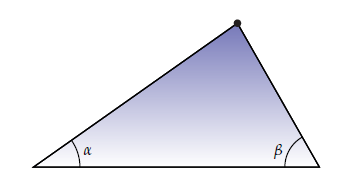
\includegraphics{images/fem_cotan_lemma3.PNG}
        \caption{\cite[p. 106]{book::DDG}}
    \end{figure}
\end{lemma}

\begin{proof}
    %\url{https://graphics.stanford.edu/courses/cs468-13-spring/assets/lecture12-lu.pdf}
    
    We have
    
    \begin{align*}
        \langle \hnabla \phi, \hnabla \phi \rangle
        = \int_{\text{triangle}} (\hnabla \phi) \cdot (\hnabla \phi)
        = \int_{\text{triangle}} ||\hnabla \phi||^2
        = A ||\hnabla \phi||^2,
    \end{align*}
    
    where $A$ is the area of the triangle. In the proof of the previous theorem, we showed $||\hnabla \phi|| = \frac{1}{h}$, where $h$ is the height of the triangle. So
    
    \begin{align*}
        \langle \hnabla \phi, \hnabla \phi \rangle
        = \frac{A}{h^2} 
        = \frac{\frac{1}{2}||\ee||h}{h^2} 
        = \frac{1}{2} \frac{||\ee||}{h}.
    \end{align*}
    
    Apply Lemma \ref{ch::ddg:lemma::cotan_w_h_lemma}, which states that the width-height ratio $\frac{||\ee||}{h}$ is $\frac{||\ee||}{h} = \cot(\alpha) + \cot(\beta)$, to obtain the result.
\end{proof}

\begin{lemma}
\label{ch::ddg::lemma::cotan_4}
    (Cotan formula lemma 4).
    
    Consider the hat functions $\phi_{\pp_i}$ and $\phi_{\pp_j}$ corresponding to vertices $\pp_i$ and $\pp_j$ of the same triangle. We have
    
    \begin{align*}
        \langle \hnabla \phi_{\pp_i}, \hnabla \phi_{\pp_j} \rangle = - \frac{1}{2} \cot(\theta),
    \end{align*}
    
    where $\theta$ is the angle between opposing edge vectors.
    
    \begin{figure}[H]
        \centering
        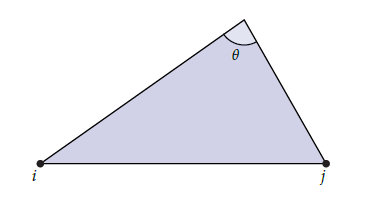
\includegraphics{images/fem_cotan_lemma4.PNG}
        \caption{\cite[p. 106]{book::DDG}}
    \end{figure}
\end{lemma}

\begin{proof}
    We have
    
    \begin{align*}
        \langle \hnabla \phi_{\pp_i}, \hnabla \phi_{\pp_j} \rangle
        = \int_{\text{triangle}} (\hnabla \phi_{\pp_i}) \cdot (\hnabla \phi_{\pp_i})
        = A (\hnabla \phi_{\pp_i}) \cdot (\hnabla \phi_{\pp_i}),
    \end{align*}
    
    where $A$ is the area of the triangle. Applying Lemma \ref{ch::ddg:lemma::cotan_edge_perp}, we have $\hnabla \phi_{\pp_i} = \frac{(\ee_{\pp_i})_\perp}{2A}$ and $\hnabla \phi_{\pp_j} = \frac{-(\ee_{\pp_j})_\perp}{2A}$, so
    
    \begin{align*}
        \langle \hnabla \phi_{\pp_i}, \hnabla \phi_{\pp_j} \rangle
        = A \frac{(\ee_{\pp_i})_\perp}{2A} \cdot \frac{-(\ee_{\pp_j})_\perp}{2A}
        = -\frac{\ee_{\pp_i} \cdot \ee_{\pp_j}}{4A}
        = -\frac{||\ee_{\pp_i}|| ||\ee_{\pp_j}|| \cos(\theta)}{4A}.
    \end{align*}
    
    To complete the proof, we do some trigonometry. Let $h$ be the height of the triangle, let $\alpha$ be the angle at vertex $\pp_i$ and let $\beta$ be the angle at vertex $\pp_j$. Then
    
    \begin{align*}
        \langle \hnabla \phi_{\pp_i}, \hnabla \phi_{\pp_j} \rangle
        = -\frac{||\ee_{\pp_i}|| \spc ||\ee_{\pp_j}|| \cos(\theta)}{4A}
        = -\frac{\frac{h}{\sin(\beta)} \frac{h}{\sin(\alpha)} \cos(\theta)}{4(\frac{1}{2}wh)}
        = -\frac{h \cos(\theta)}{2w\sin(\alpha)\sin(\beta)}
    \end{align*}
    
    where $w$ is the length of the base of the triangle. From Lemma \ref{ch::ddg:lemma::cotan_w_h_lemma}, we know ${w = h(\cot(\alpha) + \cot(\beta))}$. Thus, the above becomes
    
    \begin{align*}
        \langle \hnabla \phi_{\pp_i}, \hnabla \phi_{\pp_j} \rangle
        &= -\frac{\cos(\theta)}{2(\cot(\alpha) + \cot(\beta))\sin(\alpha)\sin(\beta)}
        = -\frac{\cos(\theta)}{2 \Big( \frac{\cos(\alpha)}{\sin(\alpha)} + \frac{\cos(\beta)}{\sin(\beta)}\Big) \sin(\alpha)\sin(\beta)} \\
        &= - \frac{\cos(\theta)}{2(\cos(\alpha) \sin(\beta) + \cos(\beta) \sin(\alpha))} = -\frac{\cos(\theta)}{2\sin(\alpha + \beta)}.
    \end{align*}
    
    Since $\alpha + \beta = \theta$, we obtain the claimed result. 
\end{proof}

Recall, the purpose of these lemmas was to determine $\langle \phi_{\pp_i}, \phi_{\pp_j} \rangle$. We needed to determine $\langle \phi_{\pp_i}, \phi_{\pp_j} \rangle$ so that we can finish the computation from the end of Derivation \ref{ch::ddg::deriv::discrete_laplacian_inner_prod_grad}:

\begin{align*}
    \langle \hDelta h, \phi_{\pp_i} \rangle
     = \sum_j ([h]_\Phi)_j \langle \hnabla \phi_{\pp_j}, \hnabla \phi_{\pp_i} \rangle.
\end{align*}

Lemma \ref{ch::ddg::lemma::cotan_3} gives us a formula for $\langle \phi_{\pp_i}, \phi_{\pp_j} \rangle$ when $i = j$, and Lemma \ref{ch::ddg::lemma::cotan_4} gives us a formula for $\langle \phi_{\pp_i}, \phi_{\pp_j} \rangle$ when $i \neq j$. Plugging the results of these lemmas into the above sum, we obtain the following theorem.

\begin{theorem}
    (Cotan formula via FEM).
    
    \begin{align*}
        (\hDelta h)_{\pp_i} = \frac{1}{2} \sum_j \Big( \cot(\alpha_j) - \cot(\beta_j) \Big) (h|_{\pp_i} - h|_{\pp_j})
    \end{align*}
\end{theorem}

\subsubsection*{Discretizing the Laplacian with discrete differential geometry}

We now use discrete differential geometry to produce a nearly identitical discretization for the Laplacian (the $\hDelta$ derived in this section will differ from the $\hDelta$ derived with the finite element method by a scalar multiple).

\begin{defn}
    (Discrete Laplacian via discrete differential geometry).
    
    Let $K$ be a $2$-mesh embedded in $\R^3$. Since Theorem \ref{ch::diff_forms::thm::div_grad_curl_exterior_derivative} tells us that $\text{div}(\VV) = *d*\VV^\flat$ and $\text{grad}(f) = (df)^\sharp$, then the ``regular'' Laplacian must act on $f$ by $\Delta f = (*d*d)f$. Thus, the ``regular'' Laplacian is
    
    \begin{align*}
        \Delta = *d*d.
    \end{align*}
    
    This ``regular'' Laplacian is easily discretized- to discretize, we just put hats on the $*$'s and $d$'s! Formally, the \textit{discrete Laplacian (via discrete differential geometry)} is defined to be
    
    \begin{align*}
        \hDelta := \hst \spc \spc \ddual \spc \spc \hst \spc \spc \dprimal,
    \end{align*}
    
    where $\dprimal$ and $\ddual$ are the discrete exterior derivatives on the primal and dual meshes, respectively. Referring back to Definition \ref{ch::ddg::defn::discrete_hodge_dual}, we see that the rightmost $\hst$ must be the diagonal Hodge-dual and that the leftmost $\hst$ must be the inverse of the third definition of the Hodge-dual from Definition \ref{ch::ddg::defn::discrete_hodge_dual}.
\end{defn}

\begin{theorem}
    (Formula for the discrete Laplacian on a $2$-mesh embedded in $\R^3$).

    Let $K$ be a $2$-mesh embedded in $\R^3$, and consider a discrete differential $0$-form $\hf$ on $K$. Then 
    
    \begin{align*}
        \boxed
        {
            (\hDelta \hf)_{\pp_i} = (\hst \spc \ddual \spc \hst \spc \dprimal \spc \hf)_{\pp_i} = \frac{1}{|\pp_i^*|} \sum_j \frac{|e_{ij}^*|}{|e_{ij}|}(f|_{\pp_j} - f|_{\pp_i})
        }
    \end{align*}
    
    where $\pp_i^*$ is the $2$-cell in the dual mesh that is dual to the vertex $\pp_i$ in the primal mesh $K$.
\end{theorem}

\begin{proof}
    First, we evaluate $\hd \hf$ on an arbitrary edge extending from $\pp_i$; let $e_{ij}$ be the edge connecting vertices $\pp_i$ and $\pp_j$ that has the standard orientation of $\{\pp_i, \pp_j\}$ inherited from $\R^2$. To take the discrete exterior derivative $\dprimal$, we integrate along the single edge $e_{ij}$:
    
    \begin{align*}
        (\dprimal \hf)_{e_{ij}} = \int_{e_{ij}} df = \int_{\pd e_{ij}} f = f|_{\pp_j} - f|_{\pp_i}.
    \end{align*}
    
    Then, applying the diagonal Hodge-dual $\hst$, we have
    
    \begin{align*}
        (\hst \spc \dprimal \hf)_{e_{ij}} 
        = \frac{|e_{ij}^*|}{|e_{ij}|}(f|_{\pp_j} - f|_{\pp_i}).
    \end{align*}
    
    Here, $e_{ij}^*$ is the $1$-cell that is dual to the $1$-simplex (the edge) $e_{ij}$. 
    
    Next, we apply $\ddual$ to $\hst \spc \dprimal \hf$. To do so, we only have to observe that $\ddual(\hst \spc \dprimal \hf)$ will be evaluated at the $2$-cell $\pp_i^*$ in the dual mesh; Stokes' theorem for discrete differential forms (Theorem \ref{ch::ddg::thm::discrete_stokes}) takes care of the rest:
    
    %\begin{align*}
    %    (\ddual \spc \hst \spc \dprimal \spc \hf)_C = \int_C d(*df).
    %\end{align*}
    
    %The $*df$ in the integrand on the right hand side, $d(*df)$, can be thought of as the result of taking the hats and subscripts off of the symbols in ``$\hst \spc \dprimal \hf$''. This corresponds to going from discrete differential geometry to ``regular'' differential geometry. 
    
    %Using Stokes' theorem for discrete differential forms (recall Theorem \ref{ch::ddg::thm::discrete_stokes}), the integral becomes
    
    \begin{align*}
       (\ddual \spc \hst \spc \dprimal \spc \hf)_{\pp_i^*}
       = \sum_j \frac{|e_{ij}^*|}{|e_{ij}|}(f|_{\pp_j} - f|_{\pp_i}).
    \end{align*}
    
    The last Hodge-dual is the inverse of the third Hodge-dual presented in Definition \ref{ch::ddg::defn::discrete_hodge_dual}. Thus, applying the last Hodge-dual divides the previous result by the area of $|\pp_i^*|$, and we obtain the claimed result.
\end{proof}

We only need one more lemma to complete our discretization of the Laplacian with discrete differential geometry.

\begin{lemma}
    (Cotan formula lemma).
    
    \begin{figure}[H]
        \centering
        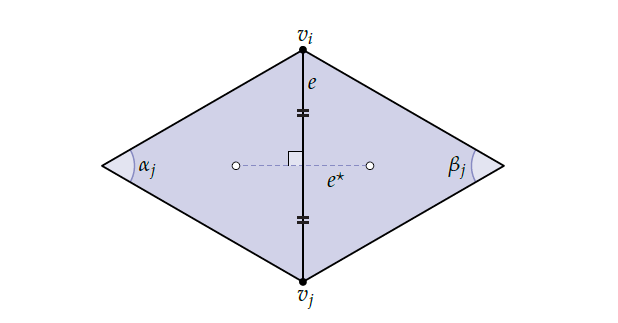
\includegraphics{images/DEC_cotan_formula.PNG}
        \caption{The diagram, which is from \cite[p. 110]{book::DDG}, uses $e$ and $e^*$ to denote $e_{ij}$ and $e_{ij}^*$.}
    \end{figure}
    
    Since Lemma \ref{ch::ddg:lemma::cotan_w_h_lemma} shows that the width-height ratio $\frac{2|e_{ij}^*|}{|e_{ij}|}$ is $\frac{2|e_{ij}^*|}{|e_{ij}|} = \cot(\alpha_j) + \cot(\beta_j)$, then
    
    \begin{align*}
        \frac{|e_{ij}^*|}{|e_{ij}|} = \frac{1}{2}(\cot(\alpha_j) + \cot(\beta_j)).
    \end{align*}
\end{lemma}

Combining the previous lemma and theorem, we obtain the following theorem, which finalizes our differential geometric discretization of the Laplacian.

\begin{theorem}
    (Cotan formula via discrete differential geometry).
    
    \begin{align*}
        \boxed
        {
            (\hDelta \hf)_{\pp_i} = \frac{1}{2 |\pp_i^*|} \sum_j \Big( \cot(\alpha_j) + \cot(\beta_j) \Big) (\hf|_{\pp_j} - \hf|_{\pp_i})
        }
    \end{align*}
    
\end{theorem}

\subsection*{Solving the problem}

We've seen that the discrete Laplacian can be expressed using the ``cotan formula'', and that this ``cotan formula'' can be derived using either the finite element method or with discrete differential geometry. How do we use this formula in a computer to smooth out surfaces in real time? The following theorem helps with this.

\begin{theorem}
    (Cotangent of the angle between vectors).
    
    Let $\vv_1, \vv_2 \in \R^3$, and consider the angle $\theta$ between $\vv_1$ and $\vv_2$. We have
    
    \begin{align*}
        \cot(\theta) = \frac{\vv_1 \cdot \vv_2}{||\vv_1 \times \vv_2||}.
    \end{align*}
\end{theorem}

\begin{proof}
    By definition of $\cot$, $\cot(\theta) = \frac{||(\vv_1)_{||}||}{||(\vv_1)_\perp||}$. Using Lemma \ref{ch::lin_alg::thm::vector_proj_dot_product}, we have $||(\vv_1)_{||}|| = ||\proj(\vv_1 \rightarrow \vv_2)|| = \frac{\vv_1 \cdot \vv_2}{||\vv_2||}$. Also, $||\vv_1 \times \vv_2|| = ||(\vv_1)_\perp|| ||\vv_2||$, so $||(\vv_1)_\perp|| = \frac{||\vv_1 \times \vv_2||}{||(\vv_1)_\perp||}$. Combining these two facts, we obtain $\cot(\theta) = \frac{(\vv_1 \cdot \vv_2)/||\vv_2||}{||\vv_1 \times \vv_2||/||\vv_2||}$, so $\cot(\theta) = \frac{\vv_1 \cdot \vv_2}{||\vv_1 \times \vv_2||}$.
\end{proof}

This theorem guarantees that if all lengths of all edges in our mesh are all the same, then the cotangent of the angle between any two edge vectors is a bilinear function. More specifically, since the cotangent produces a scalar, the cotangent of the angle between edges is a bilinear form in this situation. We learned in Chapter \ref{ch::bilinear_forms_metric_tensors} that a bilinear form can be identified with a $\binom{1}{1}$ tensor. Thus, provided that the edge lengths are all the same, we can produce a matrix which describes the action of the discrete Laplacian at each vertex.

\newpage

\section{Surface parameterization}

In this section, we explore how to wrap a $2$-dimensional map onto a $3$-dimensional surface (such as a globe) in an angle preserving manner\footnote{Our ``wrapping'' will not preserve lengths.}. Actually, instead of wrapping a $2$-dimensional map onto a $3$-dimensional surface, we will think about \textit{unwrapping} a $3$-dimensional surface into a flat $2$-dimensional map. That is, we will be considering smooth charts (recall Definition \ref{ch::manifolds::defn::chart}) on a $3$-dimensional manifold that map into a $2$-dimensional space.

Since we are dealing with the problem of angle-preservation, we will need to deal with rotations in the ``flat'' unwrapped domain. One easy way to deal with such $2$-dimensional rotations is to use the complex numbers $\C$, since multiplying by $i = \sqrt{-1}$ corresponds to performing a counterclockwise rotation by $\frac{\pi}{2}$ in the complex plane. Thus, given a smooth $2$-manifold $M$ embedded in $\C$, we will look for a global smooth chart $z:M \rightarrow \C$ that is angle preserving.

Before we proceed looking for such $z:M \rightarrow \C$, we need to define \textit{complex differential forms}.

\begin{defn}
    (Complex differential $k$-form).
    
    Earlier, we defined a \textit{real} differential $k$-form on a smooth manifold WWBOC $M$ to be a continuous function $\Lambda^k(T^*(M)) \rightarrow M$, where $\Lambda^k(T^*(M))$ is the subset of $T^0_k(T(M))$ consisting of antisymmetric tensors. These differential forms were \textit{real} in the sense that $T_\pp^*(M)$ was considered the double dual to the vector space $C^\infty(M \rightarrow \R)$. (This consideration ripples upwards because $T^*(M) := \bigsqcup_{\pp \in M} T_\pp^*(M)$).
    
    Let $M$ be a smooth manifold WWBOC. A \textit{complex} differential $k$-form on $M$ is a continuous function $\Lambda^k(T^*(M)) \rightarrow M$, where $\Lambda^k(T^*(M))$ is the subset of $T^0_k(T(M))$ consisting of antisymmetric tensors, and where $T_\pp^*(M)$ is considered as the double dual to the vector space $C^\infty(M \rightarrow \C)$.
    
    In practical terms, this definition implies the following analogue of Theorem \ref{ch::diff_forms::theorem::diff_form_in_chart}. Let $M$ be a smooth manifold WWBOC. Given any smooth chart $(U, \xx)$ on $M$, where $x^i$ is the $i$th component function of $\xx$, a complex differential $k$-form $\omega$ can be expressed as

    \begin{align*}
        \omega = \sum_{1 \leq i_1 < ... < i_k \leq n} (f_{i_1...i_k} + i g_{i_1 ... i_k}) dx^{i_1} \wedge ... \wedge dx^{i_k},
    \end{align*}
    
    where each $f_{i_1...i_k}, g_{i_1...i_k}:U \rightarrow \R$.
\end{defn}

Now that we have defined complex differential forms, we are able to speak of the differential of a complex-valued function. This is necessary for formally defining what it means for a chart on a smooth $2$-manifold embedded in $\C$ to preserve angles.

\begin{defn}
    (Angle-preserving complex chart).
    
    Let $M$ be a smooth $2$-manifold embedded in $\C$. A chart $z:M \rightarrow \C$ is \textit{angle-preserving} iff the following condition is satisfied:
    
    \begin{align*}
        \hat{\nn} \times dz(v_\pp) = i dz(v_\pp) \text{ for all $v_\pp \in T_\pp(M)$}.
    \end{align*}
    
    The left side is the result of pushing forward a tangent vector with the differential of $z$ and then rotating that tangent vector counterclockwise by $\frac{\pi}{2}$. The right side is the same thing, but the rotation has just been expressed using multiplication by $i$ rather than with a cross product.
\end{defn}

We now turn the above condition into one that is stated in terms of differential geometric concepts. This is accomplished by the following theorem, definition, and theorem.

\begin{theorem}
    (Cauchy-Riemann equation).

    Let $M$ be as in the previous definition, and suppose $z:M \rightarrow \C$ is angle-preserving. Notice that instead of pushing $v_\pp$ forward by $dz$ and then rotating with the cross product, we could have rotated and \textit{then} pushed forward $v_\pp$ with $dz$. More formally, there must be some $J:T_\pp(M) \rightarrow T_\pp(M)$ for which $\hat{\nn} \times d\FF(v_\pp) = d\FF(J(v_\pp))$. Thus, the definition of an angle preserving chart is equivalent to

    \begin{align*}
        dz(J(v_\pp)) = idz(v_\pp) \text{ for all $v_\pp \in T_\pp(M)$}.
    \end{align*}
    
    This equation is known as the \textit{Cauchy-Riemann equation}.
\end{theorem}

To obtain a differential geometric statement of the Cauchy-Riemann equation, we need to define the \textit{complex Hodge-dual}, which acts on complex differential forms.

\begin{defn}
    (Complex Hodge-dual).

    Let $M$ be a smooth $2$-manifold embedded in $\C$, and consider complex differential forms on $M$. We define the complex Hodge-dual $*$ to act on complex differential $1$- and $2$- forms, as follows. To specify the action of the complex Hodge-dual, we treat differential forms as objects that, pointwise, are functions. (Recall Derivation \ref{ch::diff_forms::deriv::diff_forms_actual_fns}).
    
    Let $v_\pp$ be any tangent vector with\footnote{Since the smooth $2$-manifolds we are considering are embedded in $\C$, their tangent spaces at any point can be identified with $\C$. The length of a tangent vector is then computed using the norm induced by the analogue of the dot product for $\C$. See example \ref{ch::ddg::example::complex_dot_prod}.} unit length.
    
    \begin{align*}
        &*\omega(v_\pp) := \omega(J(v_\pp)), \quad \text{$\omega$ is a complex differential $1$-form} \\
        &*\omega := \omega(v_\pp, J(v_\pp)), \quad \text{$\omega$ is a complex differential $2$-form}
    \end{align*}
    
    As a sanity check, note that the complex Hodge-dual of a complex differential $1$-form is a complex differential $(2 - 1 = 1)$-form, and the complex Hodge-dual of a complex differential $2$-form is a complex differential $(2 - 2 = 0)$-form.
\end{defn}

We can now present our final restatement of the angle-preservation condition.

\begin{theorem}
    (Cauchy-Riemann with the Hodge-dual).

     Let $M$ be a smooth $2$-manifold embedded in $\C$. The Cauchy-Riemann equation is
     
     \begin{align*}
        dz(J(v_\pp)) = idz(v_\pp) \text{ for all $v_\pp \in T_\pp(M)$}.
    \end{align*}
    
    The left hand side can be written as a contraction: $dz(J(v_\pp)) = C(dz, J(v_\pp))$. Using the previous definition of the complex Hodge-dual, we have $C(dz, J(v_\pp)) = C(*dz, v_\pp)$. Then, converting back to evaluation by the differential, we have $C(*dz, v_\pp) = *dz(v_\pp)$. Thus, the above is
    
    so the above becomes
    
    \begin{align*}
        *dz(v_\pp) = idz(v_\pp) \text{ for all $v_\pp \in T_\pp(M)$}.
    \end{align*}
    
    So the Cauchy-Riemann equation is equivalent to
    
    \begin{align*}
        \boxed
        {
            *dz = idz
        }
    \end{align*}
\end{theorem}

Having successfully translated the condition for angle-preservation into differential geometric terms, we will now find charts $z:M \rightarrow \C$ that ``almost'' solve the Cauchy-Riemann equation; we find charts that are as close to angle-preserving as possible.

Just as we did in our brief encounter with the finite element method, we will minimize the normed residual $||*dz - idz||$ of a chart $z:M \rightarrow \C$ to produce the chart which fails to solve the Cauchy-Riemann equation with by the smallest margin. (This time, we will not assume that the minimum such ``margin'' is zero, however).

To do this, we need to define an inner product, so that we can use its induced norm $||\cdot||$. Since we are working with complex numbers, we will actually be defining a \textit{Hermitian inner product}, which is similar to but not exactly the same as a ``regular'' inner product.

\begin{defn}
    (Hermitian inner product).
    
    Let $V$ be a vector space over $\C$. A \textit{Hermitian inner product} on $V$ is a binary function $\langle \cdot, \cdot \rangle:V \times V \rightarrow \C$ satisfying the following properties:
    
    \begin{enumerate}
        \item $\langle \cdot, \cdot \rangle$ respects addition. That is...
        \begin{enumerate}
            \item $\langle \vv_1 + \vv_2, \vv \rangle = \langle \vv_1, \vv \rangle + \langle \vv_2, \vv \rangle$ for all $\vv, \vv_1, \vv_2 \in V$.
            \item $\langle \vv, \vv_1 + \vv_2 \rangle = \langle \vv, \vv_1 \rangle + \langle \vv, \vv_2 \rangle$ for all $\vv, \vv_1, \vv_2 \in V$.
        \end{enumerate}
        \item $\langle c \vv_1, \vv_2 \rangle = c \langle \vv_1, \vv_2 \rangle$ for all $\vv_1, \vv_2 \in V$ and $c \in \C$.
        \item $\langle \vv_1, c \vv_2 \rangle = \cj{c} \langle \vv_1, \vv_2 \rangle$ for all $\vv_1, \vv_2 \in V$ and $c \in \C$.
        \item $\langle \vv_1, \vv_2 \rangle = \cj{\langle \vv_2, \vv_2 \rangle}$ for all $\vv_1, \vv_2 \in V$.
        \item $\langle \cdot, \cdot \rangle$ is positive-definite. That is, for all $\vv \in V$, $\langle \vv, \vv \rangle \geq 0$, and $\langle \vv, \vv \rangle = \mathbf{0}$ iff $\vv = \mathbf{0}$.
    \end{enumerate}
\end{defn}

\begin{example}
\label{ch::ddg::example::complex_dot_prod}
    The traditional example of a Hermitian inner product on an $n$-dimensional vector space $V$ over $\C$ is following ``complex analogue'' of the dot product: $\langle \vv_1, \vv_2 \rangle := \sum_{i = 1}^n ([\vv_1])^i \cj{([\vv_2])^i}$.
\end{example}

We now define the Hermitian product on complex differential $1$-forms that we will use to measure the normed residual.

\begin{defn}
    (Hodge Hermitian inner product on complex differential $1$-forms).
    
    Let $M$ be a smooth $2$-manifold embedded in $\C$. The \textit{Hodge Hermitian inner product} $\dlangle \cdot, \cdot \drangle$ on complex differential $1$-forms is the Hermitian inner product defined as
    
    \begin{align*}
        \dlangle \omega, \eta \drangle := \text{Re} \int_M *\cj{\omega} \wedge \eta.
    \end{align*}
\end{defn}

\begin{proof}
    We will show that $\dlangle \cdot, \cdot \drangle$ is positive-definite. The other conditions are simple to check.
    
    Consider $*\cj{\omega} \twedge \omega(v_\pp, J(v_\pp))$. (Recall Derivation \ref{ch::diff_forms::deriv::diff_forms_actual_fns} for what it means to interpret a differential form as an object that is, pointwise, a function. Also recall that we use $\twedge$ rather than $\wedge$ for such differential forms). We have
    
    \begin{align*}
        *\cj{\omega} \twedge \omega(v_\pp, J(v_\pp))
        =
        \det 
        \begin{pmatrix}
            *\cj{\omega}(v_\pp) & \omega(v_\pp) \\
            *\cj{\omega}(J(v_\pp)) & \omega(J(v_\pp))
        \end{pmatrix}
        =
        \det 
        \begin{pmatrix}
            \cj{\omega}(J(v_\pp)) & \omega(v_\pp) \\
            \cj{\omega}(J^2(v_\pp)) & \omega(J(v_\pp))
        \end{pmatrix}.
    \end{align*}
    
    The last equality in the above line follows by applying the definition of the complex Hodge-dual. Then, since $J^2 = i \cdot i = -1$, we have
    
    \begin{align*}
       *\cj{\omega} \twedge \omega(v_\pp, J(v_\pp))
        =
        \det 
        \begin{pmatrix}
            \cj{\omega}(J(v_\pp)) & \omega(v_\pp) \\
            -\cj{\omega}(v_\pp) & \omega(J(v_\pp))
        \end{pmatrix}
        =
        \cj{\omega}(J(v_\pp)) \omega(J(v_\pp)) + \cj{\omega}(v_\pp) \omega(v_\pp).
    \end{align*}
    
    Overall, we have
    
    \begin{align*}
        *\cj{\omega} \twedge \omega(v_\pp, J(v_\pp))
        =
        \cj{\omega}(J(v_\pp)) \omega(J(v_\pp)) + \cj{\omega}(v_\pp) \omega(v_\pp).
    \end{align*}
    
    We claim that $\cj{\omega}(v_\pp) \omega(v_\pp) \geq 0$ for any $v_\pp$. If the claim is true, then the previous equation yields the condition
    
    \begin{align*}
        *\cj{\omega} \twedge \omega(v_\pp, J(v_\pp)) \geq 0, \text{with equality to zero only when $\omega = \mathbf{0}$}.
    \end{align*}
    
    (We have equality to zero only when $\omega = \mathbf{0}$ because a sum of nonnegative terms is zero only when all the terms are zero).
    
    If we have this condition, then we have proved $\dlangle \cdot, \cdot \drangle$ is positive-definite, as integration over $M$ ultimately resolves into the integral of $\cj{\omega} \twedge \omega(v_\pp, J(v_\pp))$.
    
    So, we must prove $\cj{\omega}(v_\pp) \omega(v_\pp) \geq 0$, where $\omega$ is a complex differential $1$-form. We can express $\omega$ and $\cj{\omega}$ in coordinates as
    
    \begin{align*}
        \omega &= h_1 dx^1 + h_2 dx^2 \\
        \cj{\omega} &= \cj{h_1} dx^1 + \cj{h_2} dx^2,
    \end{align*}
    
    where $h_1, h_2:M \rightarrow \C$ are smooth complex functions.
    
    We can directly compute $\cj{\omega} \twedge v_\pp(\omega, v_\pp)$ by using the above coordinate representations. Use the fact that $h_i \cj{h_i} = |h_i|^2$, where $|\cdot|$ denotes the norm defined by $|a + bi| = \sqrt{a^2 + b^2}$, to prove the claim.
\end{proof}

We now work towards a theorem that expresses the square of the normed residual, $||*dz - idz||^2$, in terms of the Laplacian $\Delta = -*d*d$. (So, this theorem will use a different sign convention for the Laplacian than was used in the previous section). We need a slew of lemmas to prove the theorem.

\begin{lemma}
     The complex Hodge-dual preserves this norm  induced by the Hodge Hermitian inner product $\dlangle \cdot, \cdot \drangle$. That is, for all complex differential $1$-forms $\omega$, we have $||*\omega|| = ||\omega||$.
\end{lemma}

\begin{proof}
    We defined the complex Hodge-dual by treating complex differential forms as objects that, pointwise, are functions. In this definition, the length of vectors input into a Hodge-dual'ed differential form were the same as the length of the vectors input to the original differential form. Since the norm induced by the Hodge Hermitian inner product is an integral involving $\omega$, and as an integral of a differential form can be interpreted as an integral of that differential form being evaluated on tangent vectors, this implies that the norm induced by the Hodge Hermitian inner product is invariant under $*$.
\end{proof}

\begin{lemma}
    (Green's first identity for complex differential $1$-forms).
    
    Let $M$ be a smooth $2$-manifold embedded in $\C$. If $f, g:M \rightarrow \C$ are smooth and the normal derivative of either $f$ or $g$ vanishes on the boundary, then
    
    \begin{align*}
        \dlangle df, dg \drangle = \dlangle \Delta f, g \drangle,
    \end{align*}
    
    where $\Delta = -*d*d$ is the Laplace operator on $0$-forms.
\end{lemma}

\begin{proof}
    From the proof of Lemma \ref{ch::ddg::lemma:green_first_identity}, we have
    
    \begin{align*}
        \int_{\pd M} g * df =  \int_M dg \wedge *df + \int_M g *\Delta f.
    \end{align*}
    
    The boundary term vanishes by assumption, so we have
    
    \begin{align*}
        0 = \int_M dg \wedge *df + \int_M g *\Delta f = -\int_M *df \wedge dg + \int_M (*\Delta f) g = -\dlangle df, dg \drangle + \dlangle \Delta f, g \drangle.
    \end{align*}
\end{proof}

\begin{lemma}
    Let $||\cdot||$ be the norm induced by the Hodge Hermitian inner product $\dlangle \cdot, \cdot \drangle$ on complex differential $1$-forms. We have
    
    \begin{align*}
        ||*dz - idz||^2 = 2 \Big( \dlangle \Delta z, z \drangle - i \int_M d\cj{z} \wedge dz \Big).
    \end{align*}
\end{lemma}

\begin{proof}
    If $\langle \cdot, \cdot \rangle$ is a Hermitian inner product, then $||z + w||^2 = \langle z + w, z + w \rangle = \langle z, z \rangle + \langle z, w \rangle + \langle w, z \rangle + \langle w, w \rangle = ||z||^2 + \langle z, w \rangle + \cj{\langle z, w \rangle} + ||w||^2 = ||z||^2 + 2\text{Re}(\langle z, w \rangle) + ||w||^2$. Applying this fact to our situation, we have $||*dz - idz||^2 = ||*dz||^2 + 2\text{Re} \dlangle *dz, -idz \drangle + ||dz||^2$. Next, we use $||*dz|| = ||dz||$ to obtain $||*dz - idz||^2 = 2(||dz||^2 + \dlangle *dz, -i dz \drangle)$. 
    
    To finish, first note that $||dz||^2 = \langle dz, dz \rangle = \langle \Delta z, z \rangle$ by Green's first identity for complex differential $1$-forms. We now handle $\dlangle *dz, -i dz \drangle$ to complete the proof. By definition, 
    
    \begin{align*}
        \dlangle *dz, -i dz \drangle = \text{Re} \int_M **\cj{dz} \wedge (- i dz).
    \end{align*}
    
    From the definition of complex Hodge-dual, $**dz = dz$. It's simple to check that $\cj{dz} = d\cj{z}$ (ultimately this is because $\cj{df} = d\cj{f}$ for a complex differential $0$-form $f$), so we have
    
    \begin{align*}
        \dlangle *dz, -i dz \drangle = \text{Re} \int_M d\cj{z} \wedge (- i dz) = -i \int_M d\cj{z} \wedge dz.
    \end{align*}
    
    This proves the theorem.
\end{proof}

\begin{lemma}
    Let $M$ be a smooth $2$-manifold embedded in $\C$. If $z:M \rightarrow \C$ is a complex differential $1$-form on $M$, then
    
    \begin{align*}
        A(z) = -\frac{i}{2} \int_M d \cj{z} \wedge dz.
    \end{align*}
    
    is the surface area of $M$.
\end{lemma}

\begin{proof}
    We need to show $-\frac{i}{2} d\cj{z} \wedge dz = dx \wedge dy$. We show the equivalent statement $d\cj{z} \wedge dz = -2i dx \wedge dy$:
    
     \begin{align*}
        d\cj{z} \wedge dz &= d(\cj{x + iy}) \wedge d(x + iy) = d(x - iy) \wedge d(x + iy) = (dx - idy) \wedge (dx + idy) \\
        &= dx \wedge dx + i  dx \wedge dy - i  dy \wedge dx + dy \wedge dy = i  dx \wedge dy - i  dy \wedge dx = 2i  dx \wedge dy.
    \end{align*}
\end{proof}

Finally, we are ready to present an expression for square of the normed residual, $||*dz - idz||^2$, in terms of the Laplacian $\Delta = -*d*d$.

\begin{theorem}
    Let $||\cdot||$ be the norm induced by the Hodge Hermitian inner product $\dlangle \cdot, \cdot \drangle$ on complex differential $1$-forms. We have

    \begin{align*}
        ||*dz - idz||^2 = 2\dlangle \Delta z, z \drangle - 4A(z),
    \end{align*}
    
    where $A(z)$ is the surface area of $M$, 
    
    \begin{align*}
        A(z) = -\frac{i}{2} \int_M d \cj{z} \wedge dz.
    \end{align*}
\end{theorem}

\begin{proof}
    Combine the previous lemma and theorem.
\end{proof}

Recall that $||*dz - idz||$ measures how much a map $z$ fails to be angle-preserving. We want to minimize $||*dz - idz||$, i.e., minimize $||*dz - idz||^2$, to produce charts which are as close as possible to being perfectly angle-preserving.

According to \cite[p. 126]{book::DDG}, the trick to solving this minimization problem is to pick appropriate constraints. We don't want to pick constraints that are too loose, and we don't want to pick constraints that are too rigid. An example of a constraint that is too rigid is that of fixing the boundary of $M$. Why is this constraint ``too rigid''? Well, since $d\cj{z} \wedge dz = d(\cj{z} dz)$, we can use Stokes' theorem to express $A(z)$ as an integral over the boundary:

\begin{align*}
    A(z) = -\frac{i}{2} \int_M d \cj{z} \wedge dz = -\frac{i}{2} \int_M d(\cj{z} dz) = -\frac{i}{2} \int_{\pd M} \cj{z} dz.
\end{align*}

If the boundary is fixed, then $A(z)$ is a constant, so minimizing $||*dz - idz||^2 = 2\dlangle \Delta z, z \drangle - 4A(z)$ is the same as minimizing $\dlangle \Delta z, z \drangle$. But $\dlangle \Delta z, z \drangle$ is positive and quadratic, so the minimum of $\dlangle \Delta z, z \drangle$ occurs when $\nabla z = \mathbf{0}$, i.e., when $\Delta z = \div(\nabla z) = 0$. The fix proposed by \cite{book::DDG} is to solve the following minimization problem:

\begin{align*}
    \min_z & ||*dz - idz|| \\
    \st &||z|| = 1 \text{ for all $z$} \\
    &\langle z, \mathbf{1} \rangle = 0 \text{ for all $z$}
\end{align*}

Since $\Delta$ can be shown to be a self-adjoint operator, the above minimization problem can be solved using eigenvalue methods. Once this minimization problem is solved, a map that is as close to angle-preserving as possible is obtained.

%\section{Vector field decomposition and design}

%\begin{itemize}
%    \item Define $\coker(\FF) := W - \im(\FF)$. Prove that $\coker(\FF) = \im(\FF)^\perp$.
%    \item Define chain complex to be a sequence of vector spaces and a sequence of linear maps
    
%    \begin{align*}
%        V_k \overset{\FF_{k - 1}}{\leftarrow} ... \overset{\FF_1}{\leftarrow} V_1
%    \end{align*}
    
%    for which $\FF_{i + 1} \circ \FF_{i} = \mathbf{0} \iff \im(\FF_{i + 1}) \subseteq \ker(\FF_i)$.
    
%    \item (Lemma). Cokernel is the kernel of the adjoint.
%    \item For a chain complex with two maps and three vector spaces we have $\im(\FF_1) \cap \im(\FF_2^*) = \{\mathbf{0}\}$, where $*$ denotes the adjoint, not the dual
%    \begin{itemize}
%        \item Prove by using the lemma and that $\FF_{i + 1} \circ \FF_{i} = \mathbf{0}$ for a chain complex
%    \end{itemize}
%    \item For a chain complex of two maps, $V = \im(\FF_1) \oplus \im(\FF_2^*) \oplus \Big( (\ker(\FF_2) - \im(\FF_1)) \bigcup \{\mathbf{0}\} \Big)$
%    \begin{itemize}
%        \item Use $(V_1 \bigcup V_2)^\perp = V_1^\perp \cap V_2^\perp$
%    \end{itemize}
%\end{itemize}
